\chapter{Calcul des coefficients pour une sphère}
\label{sec:sphere}
\minitoc
\newpage
\sectionstar{Introduction}
Après le cylindre, nous présentons la sphère, qui possède une courbure dans les deux directions.

\section{Cas d'un objet sphérique}

    Les champs solutions de Maxwell dans le cas d'un repère sphérique sont décomposables en harmoniques sphériques. Nous rappelons d'abord l’expression de ces dernières puis nous donnerons l'expression du symbole de l'opérateur de d'impédance de la même manière que \cite{cheng_spectral_1993}.

    \subsection{Les harmoniques sphériques}

        \begin{TODO}
          Mettre ici la démonstration des harmoniques sphériques? Ou une référence vers annexe ?
        \end{TODO}

        On définit les harmoniques sphériques les solutions de \(\Delta U + k^2 U = 0 \). Ce sont les fonctions \(Y_{m,n} = C(m,n) e^{im\phi}\PP^m_n(\cos \theta) \) avec \(C(m,n)\)\footnote{D’après \cite[p.~24]{nedelec_acoustic_2001}, \( C(m,n) = (-1)^m\sqrt{\frac{2n+1}{4\pi}\frac{(n-m)!}{(n+m)!}}\)} tel que
        \[
         \ds\int_S Y_{m,n} \conj{Y_{p,q}} ds = \delta_m^p \delta_n^q
        \]


        On définit les vecteurs harmonique sphériques\(\gls{phy-Mmn} ,\gls{phy-Nmn}\) solution dans la base des coordonnées sphériques de
        \[
            \left\lbrace
                \begin{aligned}
                    \vrot \vrot \vect{U} - k^2 \vect{U} = 0\\
                    \vdiv \vect{U} = 0
                \end{aligned}
            \right.
        \]
        \begin{align}
            \label{eq:defMmn}
            \Mmn[z_n](\rtp) &:= \vrot \left( \vect{r} z_n(kr) Y_{m,n}(\tp) \right)\\
            &= z_n(kr)
            \begin{bmatrix}
                0
                \\
                \frac{im}{\sin\theta}Y_{mn}(\tp)
                \\
                - \ddr{\theta}{Y_{mn}}(\tp)
            \end{bmatrix}
        \end{align}

        \begin{align}
        \label{eq:defNnn}
          \Nmn[z_n](\rtp) &:= \frac{\vrot \Mmn[z_n]}{k}(\rtp) \\
          &= \frac{1}{kr}\begin{bmatrix}
            z_n(kr)n(n+1)Y_{mn}(\tp)
            \\
            \ddr{r}{z_n}(kr)\ddr{\theta}{Y_{mn}}(\tp)
            \\
            \ddr{r}{z_n}(kr)\frac{im}{\sin\theta}Y_{mn}(\tp)
          \end{bmatrix}
        \end{align}

        L'obtention de ces vecteurs est disponible en annexes \ref{sec:annex:harmoniques_spheriques}.

        Par définition de ces vecteurs, on a les propriétés suivantes
        \begin{prop}
            \label{prop:Mmn_Nmn_rot}
            \begin{align}
                \vrot \Mmn[z_n](\rtp) &= k\Nmn[z_n](\rtp)
                \\
                \vrot \Nmn[z_n](\rtp) &= k\Mmn[z_n](\rtp)
            \end{align}
        \end{prop}

        % Ces vecteurs harmoniques sphériques possèdent les propriétés suivantes

        % \begin{align}
        % \int_{S(0,R)} \vect{M_{m,n}^{z_n}} \cdot \conj{\vect{N_{p,q}^{z_n}}} ds &= 0
        % \\
        % \int_{S(0,R)} \vect{M_{m,n}^{z_n}} \cdot \conj{\vect{M_{p,q}^{z_n}}} ds &= \gamma_{m,n}R^2 \delta_{mp}\delta_{nq}
        % \\
        % \int_{S(0,R)} \vect{N_{m,n}^{z_n}} \cdot \conj{\vect{N_{p,q}^{z_n}}} ds &= \frac{\gamma_{m,n}}{k^2} \delta_{mp}\delta_{nq}
        % \end{align}

        On a (\cite{cheng_spectral_1993})
        \begin{multline}
            \vE(\rtp) = \sum_{n\in\ZZ}\sum_{m\in\ZZ} a_{mn} \Mmn[j_n](\rtp) + b_{mn} \Nmn[j_n](\rtp)
            \\
            + c_{mn} \Mmn[h_n](\rtp) + d_{mn} \Nmn[h_n](\rtp)
        \end{multline}

        D'après les équations de Maxwell, \(\vH = i\frac{\vrot \vE}{k\eta}\)

        \begin{multline}
            \vH(\rtp) = \frac{i}{\eta}\sum_{n\in\ZZ}\sum_{m\in\ZZ} a_{mn} \Nmn[j_n](\rtp) + b_{mn} \Mmn[j_n](\rtp)
            \\
            + c_{mn} \Nmn[h_n](\rtp) + d_{mn} \Mmn[h_n](\rtp)
        \end{multline}

        On définit alors le vecteur de \(\RR^2\) suivant ( resp. son orthogonal ), la réduction du vecteur harmonique sphérique \gls{phy-Mmn} ( resp. \gls{phy-Nmn} ) aux composantes tangentielles et indépendant du rayon:

        \begin{align}
            \label{eq:defUmn_tgt}
            \Umn(\tp) &=
            \begin{bmatrix}
                \frac{im}{\sin\theta}Y_{mn}(\tp)
                \\
                - \ddr{\theta}{Y_{mn}}(\tp)
            \end{bmatrix}
        \end{align}

        \begin{align}
        \label{eq:defNmn_tgt}
          \Umn^\perp(\tp) &=
          \begin{bmatrix}
            \ddr{\theta}{Y_{mn}}(\tp)
            \\
            \frac{im}{\sin\theta}Y_{mn}(\tp)
          \end{bmatrix}
        \end{align}


        On remarque alors que les parties tangentielles des vecteurs harmoniques sphériques peuvent s'écrire:
        \begin{align}
          \Mmn[z_n]_t(\rtp) &= z_n(kr)\Umn(\tp)
          \\
          \Nmn[z_n]_t(\rtp) &= \frac{1}{kr}\ddr{r}{z_n}(kr)\Umn^\perp(\tp)
        \end{align}

        On a alors les propriétés supplémentaires
        \begin{prop}
            \label{prop:Mmn_Nmn_vect}
            \begin{align}
              \vect{e_r} \pvect \Mmn[z_n]_t(\rtp) &= krz_n(kr)\Umn^\perp(\tp)
              \\
              \vect{e_r} \pvect \Nmn[z_n]_t(\rtp) &= -\frac{1}{kr}\ddr{r}{z_n}(kr)\Umn(\tp)
            \end{align}
        \end{prop}
        Sachant donc que les composantes tangentielles du champs \(\vE\) s'écrivent

        \begin{multline}
            \vE_t(\rtp) = \sum_{n\in\ZZ}\sum_{m\in\ZZ} a_{mn} j_n(kr)\Umn(\tp) + b_{mn} \frac{1}{kr}\ddr{r}{j_n}(kr)\Umn^\perp(\tp)
            \\
            + c_{mn} h_n(kr)\Umn(\tp) + d_{mn} \frac{1}{kr}\ddr{r}{j_n}(kr)\Umn^\perp(\tp)
        \end{multline}


        Donc \(\vJ = \vect{e_r} \pvect \vH\) s'écrit

        \begin{multline}
            \vJ(\rtp) = \frac{i}{\eta}\sum_{n\in\ZZ}\sum_{m\in\ZZ} - a_{mn} \frac{1}{kr}\ddr{r}{j_n}\Umn(\tp) + b_{mn} k r j_n \Umn^\perp(\tp)
            \\
            -  \frac{1}{kr}\ddr{r}{h_n} c_{mn} \Umn(\tp) + k r h_n d_{mn} \Umn^\perp(\tp)
        \end{multline}

        Dans la suite, pour simplifier les écritures, on utilisera la notation tilde \gls{mat-tild}, telle que \( \tilde{z_n}(k_r) = \ddr{r}{z_n}(kr) \). On omettra aussi les dépendances en \(kr\) lorsqu'il n'y a pas d’ambiguïtés.

        On réécrit alors matriciellement les expressions de \(\vE_t,\vJ\).

        \begin{equation}
            \vE_t(\rtp) = \sum_{n\in\ZZ}\sum_{m\in\ZZ}
            \begin{bmatrix}
              \Umn^\perp & \Umn
            \end{bmatrix}
            \left(
              \begin{bmatrix}
                  0 & \tilde{j_n}
                  \\
                  j_n & 0
              \end{bmatrix}
              \begin{bmatrix}
                  a_{mn}
                  \\
                  b_{mn}
              \end{bmatrix}
              +
              \begin{bmatrix}
                  0 & \tilde{h_n}
                  \\
                  h_n & 0
              \end{bmatrix}
              \begin{bmatrix}
                  c_{mn}
                  \\
                  d_{mn}
              \end{bmatrix}
            \right)
        \end{equation}


        \begin{equation}
            \vJ(\rtp) = \frac{i}{\eta kr}\sum_{n\in\ZZ}\sum_{m\in\ZZ}
            \begin{bmatrix}
                \Umn^\perp & \Umn
            \end{bmatrix}
            \left(
                \begin{bmatrix}
                    0 & (kr)^2 j_n
                    \\
                    -\tilde{j_n} & 0
                \end{bmatrix}
                \begin{bmatrix}
                    a_{mn}
                    \\
                    b_{mn}
                \end{bmatrix}
                +
                \begin{bmatrix}
                    0 & (kr)^2 h_n
                    \\
                    -\tilde{h_n} & 0
                \end{bmatrix}
                \begin{bmatrix}
                    c_{mn}
                    \\
                    d_{mn}
                \end{bmatrix}
            \right)
        \end{equation}

        \begin{defn}
            On définit les vecteurs de \(\RR^2\) \(\hat{\vE_t}(r,m,n)\) et \(\hat{\vJ}(r,m,n)\) tels que
            \begin{align}
                \vE_t(\rtp) &= \sum_{n\in\ZZ}\sum_{m\in\ZZ}
                \begin{bmatrix}
                  \Umn^\perp & \Umn
                \end{bmatrix}\hat{\vE_t}(r,m,n)
                \\
                \vJ(\rtp) &= \sum_{n\in\ZZ}\sum_{m\in\ZZ}
                \begin{bmatrix}
                  \Umn^\perp & \Umn
                \end{bmatrix}\hat{\vJ}(r,m,n)
            \end{align}
        \end{defn}

        \begin{defn}
            On définit les matrices \(\mJ_{E}(r,n),\mH_{E}(r,n),\mJ_{H}(r,n),\mH_{H}(r,n)\)
            \begin{align}
                \mJ_{E}(r,n) &=
                \begin{bmatrix}
                    0 & \tilde{j_n}(kr)
                    \\
                    j_n(kr) & 0
                \end{bmatrix}
                \\
                \mH_{E}(r,n) &=
                \begin{bmatrix}
                    0 & \tilde{h_n}(kr)
                    \\
                    h_n(kr) & 0
                \end{bmatrix}
                \\
                \mJ_{H}(r,n) &=
                \begin{bmatrix}
                    0 & (kr)^2 j_n(kr)
                    \\
                    -\tilde{j_n}(kr) & 0
                \end{bmatrix}
                \\
                \mH_{H}(r,n) &=
                \begin{bmatrix}
                    0 & (kr)^2 h_n(kr)
                    \\
                    -\tilde{h_n}(kr) & 0
                \end{bmatrix}
            \end{align}
        \end{defn}

        On peut donc expliciter les vecteurs précédemment introduits

        \begin{equation}
            \hat{\vE_t}(r,m,n) =
            \mJ_{E}(r,n)
            \begin{bmatrix}
                a_{mn}
                \\
                b_{mn}
            \end{bmatrix}
            +
            \mH_{E}(r,n)
            \begin{bmatrix}
                c_{mn}
                \\
                d_{mn}
            \end{bmatrix}
        \end{equation}

        \begin{equation}
            \hat{\vJ}(r,m,n) = \frac{i}{\eta k r}
            \left(
            \mJ_{H}(r,n)
            \begin{bmatrix}
                a_{mn}
                \\
                b_{mn}
            \end{bmatrix}
            +
            \mH_{H}(r,n)
            \begin{bmatrix}
                c_{mn}
                \\
                d_{mn}
            \end{bmatrix}
            \right)
        \end{equation}

    \subsection{Symbole de l'opérateur d'impédance pour une couche}

        \begin{figure}[!hbt]
          \centering
            \tikzsetnextfilename{sphere_1_couche}
          \begin{tikzpicture}
            \tikzmath{
    \a = 80;
    \b = 100;
    \d = 0.5;
    \ri = 20;
    \re = \ri;
}

% Le conducteur
\tikzmath{
    \ri = \re;
    \re = \ri + 0.5*\d;
    \xa = cos(\a)*\re;
    \ya = sin(\a)*\re;
    \xb = cos(\b)*\ri;
    \yb = sin(\b)*\ri;
}

\coordinate (a) at (\xa,\ya);
\coordinate (b) at (\xb,\yb);

\fill [pattern=north east lines] (a) arc (\a:\b:\re) -- (b) arc (\b:\a:\ri) -- cycle;
\draw (a) arc (\a:\b:\re);
\draw (a) node [right] {$r_0$};


% Le repère
\coordinate (n) at ($(a)+(0.5,-1)$);
%
%
%\draw [->] (n) -- ++(0,1) node [at end, right] {$\v{\pr}$};
%\draw [->] (n) -- ++(1,0) node [at end, right] {$\v{\pt}$};
%
\draw (n) ++(0.2,0.2) circle(0.1cm) node [above=0.1cm] {\(\vect{e_\phi}\)};
\draw (n) ++(0.2,0.2) +(135:0.1cm) -- +(315:0.1cm);
\draw (n) ++(0.2,0.2) +(45:0.1cm) -- +(225:0.1cm);


% 1ere couche
\tikzmath{
    \ri = \re;
    \re = \ri + \d;
    \xa = cos(\a)*\re;
    \ya = sin(\a)*\re;
    \xb = cos(\b)*\ri;
    \yb = sin(\b)*\ri;
    \xc = cos(0.5*(\b+\a))*(\ri+0.5*\d);
    \yc = sin(0.5*(\b+\a))*(\ri+0.5*\d);
}

\coordinate (a) at (\xa,\ya);
\coordinate (b) at (\xb,\yb);
\coordinate (c) at (\xc,\yc);

\fill [lightgray] (a) arc (\a:\b:\re) -- (b) arc (\b:\a:\ri) -- cycle;
\draw (a) arc (\a:\b:\re);
\draw (c) node {$\nu,\eta,d$};

% Le vide
\tikzmath{
    \xc = cos(0.5*(\b+\a))*(\re);
    \yc = sin(0.5*(\b+\a))*(\re);
}

\draw (\xc,\yc) node [above] {vide};
          \end{tikzpicture}
        \end{figure}

        \begin{defn}
          On définit le symbole de l'opérateur d'impédance \(\hat{\mZ}(m,n)\) tel que
          \[
              \hat{\vE_t}(r_1,m,n) = \hat{\mZ}(m,n)\hat{\vJ}(r_1,m,n)
          \]
        \end{defn}

        En \(r=r_0\), on a la relation \(\vE_t(\rtp) = 0\) donc \(\hat{\vE_t}(r_0,m,n) = 0 \)

        \begin{equation}
            \mJ_{E}(r_0,n)
            \begin{bmatrix}
                a_{mn}
                \\
                b_{mn}
            \end{bmatrix}
            = -
            \mH_{E}(r_0,n)
            \begin{bmatrix}
                c_{mn}
                \\
                d_{mn}
            \end{bmatrix}
        \end{equation}

        On suppose que les matrices \(\mJ_{E}(r_0,n)\) et \(\mH_{E}(r_0,n)\) soient inversibles.

        \begin{TODO}
          Inversibilité \(\mJ_{E}(r,n), \mH_{E}(r,n)\)
        \end{TODO}

        \begin{equation}
            \hat{\vE_t}(r,m,n) =
            \left(
                \mH_{E}(r,n)
                -
                \mJ_{E}(r,n)
                \mJ_{E}(r_0,n)^{-1}
                \mH_{E}(r_0,n)
            \right)
            \begin{bmatrix}
                c_{mn}
                \\
                d_{mn}
            \end{bmatrix}
        \end{equation}


        \begin{equation}
            \hat{\vJ}(r,m,n) = \frac{i}{\eta}
            \left(
                \mH_{H}(r,n)
                -
                \mJ_{H}(r,n)
                \mJ_{E}(r_0,n)^{-1}
                \mH_{E}(r_0,n)
            \right)
            \begin{bmatrix}
                c_{mn}
                \\
                d_{mn}
            \end{bmatrix}
        \end{equation}

        De la même manière que pour le plan et le cylindre, on en déduit le symbole de l'opérateur d'impédance

        \begin{multline}
            \hat{\mZ}(m,n) = -i\eta
            \left(
                \mH_{E}(r_1,n)
                \mH_{E}(r_0,n)^{-1}
                -
                \mJ_{E}(r_1,n)
                \mJ_{E}(r_0,n)^{-1}
            \right)
            \\
            \left(
                \mH_{H}(r_1,n)
                \mH_{E}(r_0,n)^{-1}
                -
                \mJ_{H}(r_1,n)
                \mJ_{E}(r_0,n)^{-1}
            \right)^{-1}
        \end{multline}

        Par définition des matrices \(\mJ_E,\mH_E,\mJ_H,\mH_H\), elle sont anti-diagonale. Donc leur inverse l'est aussi. Donc le produit de l'une avec l'inverse d'une autre est une matrice diagonale. Donc le symbole de l'opérateur d'impédance est une matrice diagonale.

        \begin{equation}
            \hat{\mZ}(m,n) = -i\eta
            \begin{bmatrix}
                \frac
                {\tilde{h_n}(kr_1)\tilde{j_n}(kr_0)-\tilde{j_n}(kr_1)\tilde{h_n}(kr_0)}
                {{h_n}(kr_1)\tilde{j_n}(kr_0)-{j_n}(kr_1)\tilde{h_n}(kr_0)} & 0
                \\
                0 & \frac
                {{j_n}(kr_1){h_n}(kr_0)-{h_n}(kr_1){j_n}(kr_0)}
                {\tilde{h_n}(kr_1){j_n}(kr_0)-\tilde{j_n}(kr_1){h_n}(kr_0)}
            \end{bmatrix}
        \end{equation}

    \subsection{Symbole de l'opérateur d'impédance pour plusieurs couche}

        \begin{TODO}
            Les matrices J,H dépendent de k donc de nu qui depend de la couche. Corriger.
        \end{TODO}

        \begin{figure}[!hbt]
          \centering
            \tikzsetnextfilename{sphere_n_couche}
          \begin{tikzpicture}
            \tikzmath{
    \a = 83;
    \b = 97;
    \d = 0.5;
    \ri = 30;
    \re = \ri;
}

% Le conducteur
\tikzmath{
    \ri = \re;
    \re = \ri + 0.5*\d;
    \xa = cos(\a)*\re;
    \ya = sin(\a)*\re;
    \xb = cos(\b)*\ri;
    \yb = sin(\b)*\ri;
}

\coordinate (a) at (\xa,\ya);
\coordinate (b) at (\xb,\yb);

\fill [pattern=north east lines] (a) arc (\a:\b:\re) -- (b) arc (\b:\a:\ri) -- cycle;
\draw (a) arc (\a:\b:\re);
\draw (a) node [right] {$r_0$};

% Le repère
\coordinate (n) at ($(a)+(0.5,-1)$);
%
%
%\draw [->] (n) -- ++(0,1) node [at end, right] {$\v{\pr}$};
%\draw [->] (n) -- ++(1,0) node [at end, right] {$\v{\pt}$};
%
\draw (n) ++(0.2,0.2) circle(0.1cm) node [above=0.1cm] {$\vect{e_\phi}$};
\draw (n) ++(0.2,0.2) +(135:0.1cm) -- +(315:0.1cm);
\draw (n) ++(0.2,0.2) +(45:0.1cm) -- +(225:0.1cm);

% 1 ere couche

\tikzmath{
    \ri = \re;
    \re = \ri + \d;
    \xa = cos(\a)*\re;
    \ya = sin(\a)*\re;
    \xb = cos(\b)*\ri;
    \yb = sin(\b)*\ri;
    \xc = cos(0.5*(\b+\a))*(\ri+0.5*\d);
    \yc = sin(0.5*(\b+\a))*(\ri+0.5*\d);
}

\coordinate (a) at (\xa,\ya);
\coordinate (b) at (\xb,\yb);
\coordinate (c) at (\xc,\yc);

\fill [lightgray] (a) arc (\a:\b:\re) -- (b) arc (\b:\a:\ri) -- cycle;
\draw (a) arc (\a:\b:\re);
\draw (c) node {$\nu_1,\eta_1,d_1$};


% Des couches

\tikzmath{
    \ri = \re;
    \re = \ri + 2*\d;
    \xa = cos(\a)*\re;
    \ya = sin(\a)*\re;
    \xb = cos(\b)*\ri;
    \yb = sin(\b)*\ri;
    \xc = cos(0.5*(\b+\a))*(\ri+0.5*\d);
    \yc = sin(0.5*(\b+\a))*(\ri+0.5*\d);
}

\coordinate (a) at (\xa,\ya);
\coordinate (b) at (\xb,\yb);
\coordinate (c) at (\xc,\yc);

\fill [lightgray]    (a) arc (\a:\b:\re) -- (b) arc (\b:\a:\ri) -- cycle;
\fill [pattern=dots] (a) arc (\a:\b:\re) -- (b) arc (\b:\a:\ri) -- cycle;
\draw (a) arc (\a:\b:\re);

% n eme couche

\tikzmath{
    \ri = \re;
    \re = \ri + \d;
    \xa = cos(\a)*\re;
    \ya = sin(\a)*\re;
    \xb = cos(\b)*\ri;
    \yb = sin(\b)*\ri;
    \xc = cos(0.5*(\b+\a))*(\ri+0.5*\d);
    \yc = sin(0.5*(\b+\a))*(\ri+0.5*\d);
}

\coordinate (a) at (\xa,\ya);
\coordinate (b) at (\xb,\yb);
\coordinate (c) at (\xc,\yc);

\fill [lightgray] (a) arc (\a:\b:\re) -- (b) arc (\b:\a:\ri) -- cycle;
\draw (a) arc (\a:\b:\re);
\draw (c) node {$\nu_p,\eta_p,d_p$};

% Le vide
\tikzmath{
    \xc = cos(0.5*(\b+\a))*(\re);
    \yc = sin(0.5*(\b+\a))*(\re);
}

\draw (\xc,\yc) node [above] {vide};


          \end{tikzpicture}
        \end{figure}


        \begin{defn}
          Pour chaque couche \(p\), on définit le symbole de l'opérateur d'impédance \(\hat{\mZ}_p(m,n)\) tel que
          \[
              \hat{\vE_t}(r_p,m,n) = \hat{\mZ}_p(m,n)\hat{\vJ}(r_p,m,n)
          \]
        \end{defn}

        On résonne par récurrence: on suppose connu le symbole de l'opérateur d'impédance de la couche \(p\) et on cherche le suivant

        En \(r=r_{p}=r_0+\sum_{i=1}^p d_p\), on a la relation \( \hat{\vE_t}(r_p,m,n) = \hat{\mZ}_p(m,n)\hat{\vJ}(r_p,m,n)\) où \(\hat{\mZ}_p(m,n)\) est un matrice diagonale

        \begin{equation}
            \left(\mJ_{E}(r_p,n) - \frac{i}{\eta_p}\hat{\mZ}_p(m,n)\mJ_{H}(r_p,n) \right)
            \begin{bmatrix}
                a_{mn}
                \\
                b_{mn}
            \end{bmatrix}
            = -
            \left(\mH_{E}(r_p,n) - \frac{i}{\eta_p}\hat{\mZ}_p(m,n)\mH_{H}(r_p,n) \right)
            \begin{bmatrix}
                c_{mn}
                \\
                d_{mn}
            \end{bmatrix}
        \end{equation}

        On définit les matrices \(\mA_{J}(r,n)\) et \(\mA_{H}(r,n)\) telle que

        \begin{align}
            \mA_{J}(r,n) &= \mJ_{E}(r,n) - \frac{i}{\eta_p}\hat{\mZ}_p(m,n)\mJ_{H}(r,n)
            \\
            \mA_{H}(r,n) &= \mH_{E}(r,n) - \frac{i}{\eta_p}\hat{\mZ}_p(m,n)\mH_{H}(r,n)
        \end{align}

        On suppose que les matrices \(\mA_{E}(r,n)\) et \(\mA_{H}(r,n)\) soient inversibles.

        \begin{TODO}
          Inversibilité \(\mA_{E}(r_p,n)\) et \(\mA_{H}(r_p,n)\)
        \end{TODO}

        Par hypothèse sur \(\hat{\mZ_p}(m,n)\), ces matrices sont anti-diagonale.

        On en déduit

        \begin{equation}
            \hat{\vE_t}(r_{p+1},m,n) =
            \left(
                \mH_{E}(r_{p+1},n)
                -
                \mJ_{E}(r_{p+1},n)
                \mA_{J}(r_p,n)^{-1}
                \mA_{H}(r_p,n)
            \right)
            \begin{bmatrix}
                c_{mn}
                \\
                d_{mn}
            \end{bmatrix}
        \end{equation}


        \begin{equation}
            \hat{\vJ}(r_{p+1},m,n) = \frac{i}{\eta_p}
            \left(
                \mH_{H}(r_{p+1},n)
                -
                \mJ_{H}(r_{p+1},n)
                \mA_{J}(r_{p+1},n)^{-1}
                \mA_{H}(r_{p+1},n)
            \right)
            \begin{bmatrix}
                c_{mn}
                \\
                d_{mn}
            \end{bmatrix}
        \end{equation}

        On en déduit aisément le symbole de la couche \(p+1\)

        \begin{multline}
            \hat{\mZ}_{p+1}(m,n) = -i\eta_p
            \left(
                \mH_{E}(r_{p+1},n)
                \mA_{H}(r_p,n)^{-1}
                -
                \mJ_{E}(r_{p+1},n)
                \mA_{E}(r_p,n)^{-1}
            \right)
            \\
            \left(
                \mH_{H}(r_{p+1},n)
                \mA_{H}(r_p,n)^{-1}
                -
                \mJ_{H}(r_{p+1},n)
                \mA_{E}(r_p,n)^{-1}
            \right)^{-1}
        \end{multline}

        Pour les mêmes raisons que dans le cas d'une couche, ce symbole est diagonal. Cependant son expression n'est plus aussi simple (voir annexe \ref{sec:annex:imp_sphere} ).

  \subsection{Applications numérique}

    \begin{figure}[!hbt]
        \centering
        \tikzsetnextfilename{Z_HOPPE_62_sphere_erreur}
\begin{tikzpicture}[scale=1]
\begin{loglogaxis}[
    title={},
    ylabel={\(||\hat{\mZ}_{plan} - \hat{\mZ}_{sphere}||_2\)},
    xlabel={\(r_0/d\)},
    width=0.8\textwidth,
    xmin=0.1,
    xmax=100,
    % mark repeat=20,
    legend pos=outer north east
  ]
  \legend{TM,TE}
  \addplot [black] table [x={r0/d}, y={tm},col sep=semicolon] {csv/sphere/hoppe_p62_error.csv};
  \addplot [black,dashed] table [x={r0/d}, y={te},col sep=semicolon] {csv/sphere/hoppe_p62_error.csv};
\end{loglogaxis}
\end{tikzpicture}
        \caption{\(\eps = 6, \mu = 1, d=0.0225\text{m}, f=1\text{GHz}\)}
        \label{fig:imp_fourier:sphere:hoppe_p62:converge_rayon:error}
    \end{figure}
\section{Approximation de la matrice d'impédance pour une sphère par une CIOE}

  \subsection[Expression des opérateurs LD,LR en Fourier]{Expression des opérateurs \(\LD,\LR\) en Fourier}

    Par définition de \(\LD\), on a
    \begin{align}
      \LD \vE_t & = \vgrads{} \vdivs{} \vE_t
    \end{align}
    Or 
    \begin{align*}
      \vE_t(\rtp) &= \sum_{n\in\ZZ}\sum_{m\in\ZZ} (a_{mn} j_n + c_{mn}h_n) \Umn(\rtp) + (b_{mn} \tilde{j_n}+d_{mn} \tilde{h_n}) \Umn^\perp(\rtp)
      %\intertext{donc}
      %\LD\vE_t(\rtp) &= \sum_{n\in\ZZ}\sum_{m\in\ZZ} (a_{mn} j_n + c_{mn}h_n) \LD\Umn(\rtp) + (b_{mn} \tilde{j_n}+d_{mn} \tilde{h_n}) \LD\Umn^\perp(\rtp)
    \end{align*}

    On rappelle  les expressions des vecteurs (voir \eqref{eq:defUmn_tgt}, \eqref{eq:defNmn_tgt}) dans la base sphérique (\(\vect{e_r},\vect{e_\theta},\vect{e_\phi}\))
    \begin{align*}
      \Umn(\tp) =
      \begin{bmatrix}
          0
          \\
          \frac{im}{\sin\theta}\Pmn(\cos(\theta))e^{im\phi}
          \\
          - \ddr{\theta}{\Pmn(\cos(\theta))}e^{im\phi}
      \end{bmatrix}
      &&
      \Umn^\perp(\tp) =
      \begin{bmatrix}
        0
        \\
        \ddr{\theta}{\Pmn(\cos(\theta))}e^{im\phi}
        \\
        \frac{im}{\sin\theta}\Pmn(\cos(\theta))e^{im\phi}
      \end{bmatrix}
    \end{align*}

    On commence par calculer le divergent surfacique (cf annexe \ref{sec:annexe:div_grad_rot}) en sphérique
    \begin{align*}
      \vdivs{}\Umn(\rtp) &= \frac{1}{r\sin(\theta)} \ddr{\theta}{(\sin(\theta)\Umn_\theta)} + \frac{1}{r\sin(\theta)}\ddr{\phi}{(\Umn_\phi)}
      \\
      &=\frac{ime^{im\phi}}{r\sin(\theta)}\left( \ddr{\theta}{\Pmn(\cos(\theta))} - \ddr{\theta}{\Pmn(\cos(\theta))} \right)
      \\
      &= 0
    \end{align*}
    Donc 
    \begin{align*}
      \LD\Umn(\rtp) = 0
    \end{align*}

    Calculons maintenant l'action de \(\LD\) sur \(\Umn^\perp\)
    \begin{align*}
      \vdivs{}\Umn^\perp(\rtp) &= \frac{1}{r\sin(\theta)} \ddr{\theta}{(\sin(\theta)\Umn^\perp_\theta)} + \frac{1}{r\sin(\theta)}\ddr{\phi}{(\Umn^\perp_\phi)}
      \\
      &= \frac{e^{im\phi}}{r\sin(\theta)}
      \left(
        \ddr{\theta}{}\left(\sin(\theta)\ddr{\theta}{\Pmn(\cos(\theta))}\right) - \frac{m^2}{\sin\theta}\Pmn(\cos(\theta))
      \right)
    \end{align*}
    Or d’après \cite[\href{https://dlmf.nist.gov/14.10}{sec.~14.10}]{dlmf_nist_2019} les fonctions de Legendre sont récurrentes
    \begin{align}
      \sin(\theta)\ddr{\theta}{\Pmn(\cos(\theta))} &= (n+m)\PP_{n-1}^m(\cos(\theta)) - n\cos(\theta)\Pmn(\cos(\theta))
    \end{align}

    Donc 
    \begin{align*}
      \LD\Umn^\perp(\rtp) = -\frac{n(n+1)}{r^2}\Umn^\perp(\rtp)
    \end{align*}

    On utilise les résultats de \cite{marceaux_high-order_2000}

    \begin{align*}
      \vgrads{}\vdivs{} \Mmn[z_n]_t(r,\theta,\phi) &= 0
      \\
      \vgrads{}\vdivs{} \Nmn[z_n]_t(r,\theta,\phi) &= -\frac{n(n+1)}{r^2}\Nmn[z_n]_t(r,\theta,\phi)
    \end{align*}

    On définit \(\hat{\mLD}\) l'opérateur matriciel tel que
    \begin{align}
      \LD \vE_t (r_{ext},\theta,\phi)
      &= \frac{1}{2\pi}\sum_{n=-\infty}^\infty\sum_{m=-n}^n \hat{\mLD} \hat{\vE_t}(r_{ext},n,m)
    \end{align}

    Son expression est de ce qui précède
    \begin{equation}
      \label{eq:cylindre:fourier:LD}
      \hat{\mLD}(n,m) = -
      \begin{bmatrix}
        0 & 0
        \\
        0 & \frac{n(n+1)}{r_{ext}^2}
      \end{bmatrix}
    \end{equation}

    On reprend exactement la même méthode pour l'opérateur \(\LR\).
    Par définition de \(\LR\), on a
    \begin{align}
      \LR \vE_t & = \vrots{} \vrots{} \vE_t
    \end{align}

    On utilise les résultats de \cite{marceaux_high-order_2000}

    \begin{align*}
      \vrots{}\vrots{} \Mmn[z_n]_t(r,\theta,\phi) &= \frac{n(n+1)}{r^2}\Mmn[z_n]_t(r,\theta,\phi)
      \\
      \vrots{}\vrots{} \Nmn[z_n]_t(r,\theta,\phi) &= 0
    \end{align*}

    On définit \(\hat{\LR}\) l'opérateur matriciel tel que
    \begin{align}
      \LR \vE_t(r_{ext},\theta,\phi)
      &= \frac{1}{2\pi}\sum_{n=-\infty}^\infty\sum_{m=-n}^n \hat{\LR} \hat{\vE_t}(r_{ext},n,m)
    \end{align}

    \begin{equation}
      \hat{\mLR}(n,m) =
      \begin{bmatrix}
        \frac{n(n+1)}{r_{ext}^2} & 0
        \\
        0 & 0
      \end{bmatrix}
    \end{equation}

  \subsection{Expression de la matrice d'impédance approchée par la CI3}

    Tout comme dans le cas du plan infini, on peut donc définir \(\hat{\mZ}_{IBC}\) l’opérateur matriciel associé à la condition d'impédance.

    \begin{multline}
        \hat{\mZ}_{CI3}(n,m) = \left(\mI + b_1 \frac{\hat{\mLD}(n,m)}{k_0^2} - b_2 \frac{\hat{\mLR}(n,m)}{k_0^2} \right)^{-1}\\
        \left(a_0 \mI + a_1 \frac{\hat{\mLD}(n,m)}{k_0^2} - a_2 \frac{\hat{\mLR}(n,m)}{k_0^2}\right)
    \end{multline}

\section{Calcul des coefficient des CIOE par moindres carrés}

% Pour calculer les coefficients, nous minimisons par moindres carrés
% \begin{itemize}
%   \item dans le cas du plan infini la différence entre l'impédance \(\hat\mZ_{ex}(k_x,k_y)\) et son approximation \(\hat\mZ_{ap}(k_x,k_y)\);
%   \item dans le cas du cylindre infini la différence entre les coefficients de Fourier \(\hat\mF_{ex}(n,k_z)\) et leurs approximations \(\hat\mF_{ap}(n,k_z)\);
%   \item dans le cas de la sphère la différence entre les coefficients de Mie \(\hat\mM_{ex}(n,m)\) et leurs approximations \(\hat\mM_{ap}(n,m)\);
% \end{itemize}
% Toutes ces quantités ont été définies aux chapitres \ref{sec:chap1} et \ref{sec:chap2}

\subsection{Expression des moindre carrés dans le cadre de l'approximation plan infini pour une incidence}
  Pour toutes les CIOE, on cherche à approcher le symbole de l'opérateur d'impédance \(\hat\mZ_{ex}(k_x,k_y)\) par une matrice \(\hat\mZ_{ap}(k_x,k_y)\). Le couple \((k_x,k_y)\) est fixé.

  \begin{prop}
    Soit \(k_x,k_y\) fixés.
    Pour nos CIOE, il existe une matrice \(\mH_{k_x,k_y}(CI,\hat\mZ_{ex}(k_x,k_y))\) et un vecteur \(X(CI)\) où CI représente un vecteur de \(\CC^n\) composés des \(N_{CI}\) coefficients de la CI telles que minimiser selon la norme euclidienne
    \[
      ||\hat\mZ_{ap}(k_x,k_y)-\hat\mZ_{ex}(k_x,k_y)||^2_{eucl}
    \] 
    revient à minimiser selon une norme équivalente mais dépendante de la CI
    \[ 
      || \mH_{k_x,k_y}(CI,\hat\mZ_{ex}(k_x,k_y)) \vect{X}(CI) - b(\hat\mZ_{ex}(k_x,k_y)) ||^2_{CI}
    \]
    Les dimensions de \(\mH\) sont de \( (4,N_{CI}) \) de la CI colonnes et le vecteur colonne b à 4 coefficients et a l'expression suivante
    \begin{align}
      b(\hat{\mZ}) = \begin{bmatrix} \hat{\mZ}_{11} \\ \hat{\mZ}_{12}\\ \hat{\mZ}_{21} \\ \hat{\mZ}_{22} \end{bmatrix}
    \end{align}
  \end{prop}

  \begin{proof}
    Nous démontrons ce résultat pour la \hyperlink{ci3}{CI3} où les termes \(k_0^2\) sont omis, les matrices des autres CIOE s'en déduisent.

    Soient les matrices symétriques \(\hat\mLD, \hat\mLR\) telles que

    \begin{align}
      \hat\mLD(k_x,k_y) & = - \begin{bmatrix} k_x^2 & k_x k_y \\ k_x k_y & k_y^2 \end{bmatrix}
      \\
      \hat\mLR(k_x,k_y) & =  \begin{bmatrix} k_y^2 & -k_x k_y \\ -k_x k_y &  k_x^2 \end{bmatrix}
    \end{align}

    Par définition, on a
    \begin{align}
    ||\hat\mZ_{ap}-\hat\mZ_{ex}||^2_{eucl} &= ||\left(\mI + b_1 \hat{\mLD} - b_2 \hat{\mLR}\right)^{-1}\left(a_0\mI + a_1 \hat{\mLD} - a_2 \hat{\mLR}\right)-\hat\mZ_{ex} ||^2_{eucl}
    \\
    \intertext{Posons pour alléger les formules \(\hat{\mZ}_N = a_0\mI + a_1 \hat{\mLD} - a_2 \hat{\mLR}\) et \(\hat{\mZ}_D = \mI + b_1 \hat{\mLD} - b_2 \hat{\mLR}\)}
    ||\hat\mZ_{ap}-\hat\mZ_{ex}||^2_{eucl} &= ||\hat{\mZ}_D^{-1}\hat\mZ_N-\hat\mZ_{ex} ||^2_{eucl}
    \\
    &= ||\hat{\mZ}_D^{-1}\left(\hat{\mZ}_N-\hat{\mZ}_D\hat\mZ_{ex}\right) ||^2_{eucl}
    \\
    \intertext{On sépare alors \(\hat{\mZ}_D\) en deux parties}
    ||\hat\mZ_{ap}-\hat\mZ_{ex}||^2_{eucl} &= ||\hat{\mZ}_D^{-1}\left(\hat{\mZ}_N - \left(b_1 \hat{\mLD} - b_2 \hat{\mLR}\right)\hat\mZ_{ex} - \hat\mZ_{ex}\right)||^2_{eucl}
    \intertext{On voit alors apparaitre une nouvelle norme}
    ||\hat\mZ_{ap}-\hat\mZ_{ex}||^2_{eucl} &= ||\hat{\mZ}_N - \left(b_1 \hat{\mLD} - b_2 \hat{\mLR}\right)\hat\mZ_{ex} - \hat\mZ_{ex}||^2_{\hat{\mZ}_D^{-1}}
    \intertext{Posons \(X = \begin{bmatrix} a_0 & a_1 & a_2 & b_1 & b_2 \end{bmatrix}^\perp\), alors il existe \(\mH_{k_x,k_y}(CI3,\hat\mZ_{ex})\) telle que}
    ||\hat\mZ_{ap}-\hat\mZ_{ex}||^2_{eucl} &= ||\mH_{k_x,k_y}(CI3,\hat\mZ_{ex})X - b(\hat\mZ_{ex})||^2_{\hat{\mZ}_D^{-1}}
  \end{align}

  Ces matrices et vecteurs sont définis pour cette CIOE ainsi
    \begin{align}
        \mH_{k_x,k_y}(CI3,\hat\mZ) = \begin{bmatrix}
        1 & \hat{\mLD}_{11} & -\hat{\mLR}_{11} & -\left(\hat{\mLD}\hat\mZ\right)_{11} & \left(\hat{\mLR}\hat\mZ\right)_{11}
        \\
        0 & \hat{\mLD}_{12} & -\hat{\mLR}_{12} & -\left(\hat{\mLD}\hat\mZ\right)_{12} & \left(\hat{\mLR}\hat\mZ\right)_{12}
        \\
        0 & \hat{\mLD}_{21} & -\hat{\mLR}_{21} & -\left(\hat{\mLD}\hat\mZ\right)_{21} & \left(\hat{\mLR}\hat\mZ\right)_{21}
        \\
        1 & \hat{\mLD}_{22} & -\hat{\mLR}_{22} & -\left(\hat{\mLD}\hat\mZ\right)_{22} & \left(\hat{\mLR}\hat\mZ\right)_{22}
        \end{bmatrix}
        && X = \begin{bmatrix} a_0 \\ a_1 \\ a_2 \\ b_1 \\ b_2 \end{bmatrix}
    \end{align}
  \end{proof}

  Par exemple pour la CI4, ces matrices deviennent
  \begin{align}
      \mH_{k_x,k_y}(CI4,\hat\mZ) = \begin{bmatrix}
      1 & \hat{\mLD}_{11} & -\hat{\mLR}_{11}
      \\
      0 & \hat{\mLD}_{12} & -\hat{\mLR}_{12}
      \\
      0 & \hat{\mLD}_{21} & -\hat{\mLR}_{21}
      \\
      1 & \hat{\mLD}_{22} & -\hat{\mLR}_{22}
      \end{bmatrix}
      && X = \begin{bmatrix} a_0 \\ a_1 \\ a_2 \end{bmatrix}
  \end{align}
  Nous ne détaillerons pas les autres CI, elle se déduisent aisément.

  On remarque que la fonctionnelle est quadratique si la matrice \(M=\conj{\mH^t}{\mH}\) est hermitienne définie positive. Une matrice \(A\) est hermitienne si \(\forall x, \conj{x^t}Ax \in \RR\), elle est hermitienne positive si \(\forall x, \conj{x^t}Ax \in \RR^+\) et elle est hermitienne définie positive si \(\forall x\not=0, \conj{x^t}Ax \in \RR^{+*}\).

  On remarque que par construction, notre matrice \(M\) est hermitienne positive. Cependant, cette matrice n'est pas définie si on ne considère qu'un seul couple \(k_x, k_y\).

\subsection{Expression des moindre carrés dans le cadre de l'approximation plan infini avec un balayage en incidence}

  Pour résoudre ce problème, on se dote de suffisamment d'observations, puis pour chacune de ces observations on applique la méthode de la partie précédente. Enfin on agrège tous ces moindres carrés en une seule expression pour aboutir au problème global

  Soient \(((k_x,k_y)_i)_{i=1,N_{i}}\) une famille de couple avec \(N_{i} > N_{CI}\).

  \begin{defn}
    On définit la matrice \(\tilde{\mH}(CI)\) de taille \((4N_{i},N_{CI})\) et le vecteur \(\tilde{b}\) de taille \(4N_{i}\) tels que

  \begin{align}
    \tilde{\mH}(CI) = \begin{bmatrix}
      \mH_{k_{x1},k_{y1}} (CI,\hat\mZ(k_{x1},k_{y1}))
      \\
      \vdots
      \\
      \mH_{k_{xi},k_{yi}} (CI,\hat\mZ(k_{xi},k_{yi}))
      \\
      \vdots
      \\
      \mH_{k_{xN},k_{yN}} (CI,\hat\mZ(k_{xN},k_{yN}))
      \end{bmatrix}
    &&
    \tilde{b} = \begin{bmatrix}
     b(\hat\mZ(k_{x1},k_{y1}))
     \\ 
     \vdots 
     \\ 
     b(\hat\mZ(k_{xi},k_{yi}))
     \\
     \vdots
     \\ 
     b(\hat\mZ(k_{xN},k_{yN})
     \end{bmatrix}
  \end{align}
  \end{defn}

  Le problème des moindres carrés avec \gls{acr-csu} s'énonce:

  \begin{prop}[Moindres carrés avec CSU dans le cas plan infini]
  ~

  Trouver \(X_{CI}^*\) tel que

  \[
    X_{CI}^* = \argmin{X \in SUC(CI)} \left\lVert \tilde{\mH}(CI)X_{CI} - \tilde{b}\right\rVert^2_{\RR^{Ni}}
  \]
  \end{prop}

  On remarque que la fonctionnelle est quadratique si la matrice \(\tilde{\mM}=\conj{\tilde{\mH}^t}\tilde{\mH}\) est hermitienne définie positive. Or par construction elle est hermitienne et positive, donc il existe une minimum global si la matrice est définie (ou inversible). 

  \subsubsection{Existence du minimum pour la CI4}

  \begin{prop}
    La matrice \(\tilde{\mM}\) associé à la CI4 est inversible, donc définie, s'il existe au moins 2 couples \((k_{xi},k_{yi})\) différents.
  \end{prop}

  \begin{proof}
    Soit \(t\) le vecteur de \(\left(\RR^+\right){N_{i}}\) tel que \(t_i = k_{xi}^2 + k_{yi}^2\). On a l'expression suivante de \(\tilde{\mM}\)

    \begin{equation}
      \tilde{\mM} = \begin{bmatrix}
      2 N_{i} & -\sum_{i=1}^{N_{i}} t_i & -\sum_{i=1}^{N_{i}} t_i
      \\
      -\sum_{i=1}^{N_{i}} t_i & \sum_{i=1}^{N_{i}} t_i^2 & 0
      \\
      -\sum_{i=1}^{N_{i}} t_i & 0 & \sum_{i=1}^{N_{i}} t_i^2
      \end{bmatrix}
    \end{equation}

    Pour prouver son inversibilité, on exprime son déterminant 

    \begin{align}
      \det( \tilde{\mM}) &= 2N_{i}\left(\sum_{i=1}^{N_{i}} t_i^2\right)^2 - 2 \left( \sum_{i=1}^{N_{i}} t_i\right)^2 \left(\sum_{i=1}^{N_{i}}t_i^2\right) 
      \\
      &= 2\left(\sum_{i=1}^{N_{i}} t_i^2\right)\left(N_{i}\sum_{i=1}^{N_{i}} t_i^2 - \left( \sum_{i=1}^{N_{i}} t_i\right)^2 \right)
      \\
      \intertext{Soit \(\left<\cdot,\cdot\right>\) le produit scalaire associé à \(\RR^{N_{i}}\), alors}
      \det( \tilde{\mM}) &= 2\left<t,t\right>\left( \left<1,1\right>\left<t,t\right>- \left<t,1\right>^2\right)
    \end{align}

    Donc d'après Cauchy–Schwarz (voir \cite[\href{https://dlmf.nist.gov/1.7\#E1}{eq.~1.7.1}]{dlmf_nist_2019}), le terme de droite est non-nul pour tout \(t\) non colinéaire au vecteur dont toutes les composantes valent 1, c'est à dire n'importe quel vecteur ayant au moins deux composantes différentes.
  \end{proof}

\subsubsection{Existence du minimum pour la CI3}

  L'introduction de \(\hat\mZ_{ex}\) dans \(\tilde M\) ne permet plus d'exprimer simplement le déterminant de cette dernière. Nous n'avons pas réussi à prouver que cette matrice était définie. Cependant nous avons vérifié numériquement qu'elle l'était pour tous les empilements que nous avons testés.

% \subsection{Expression des moindre carrés dans le cadre de l'approximation cylindre pour une incidence}

  \subsection{Résultats numériques sans contraintes}

      Sans contraintes, on résout le système linéaire \(\tilde \mH X - \tilde b\). Numériquement, nous avons utilisé la routine de résolution au sens des moindres carrés \href{http://www.netlib.org/lapack/explore-html/d6/d10/group__complex16_g_esolve_ga1d8089ba1e1538eb3d1ab0ebe97596c7.html}{ZGELS}.


      Dans \cite{stupfel_implementation_2015} sont introduites les CIOE
      \begin{itemize}
        \item CI01
          \begin{equation}
            \vE_t = \left(a_0\oI + a_1\frac{\LL}{k_0^2}\right)\vJ
          \end{equation}
        \item CI1
          \begin{equation}
            \left(\oI + b\frac{\LL}{k_0^2} \right)\vE_t = \left(a_0\oI + a_1\frac{\LL}{k_0^2}\right)\vJ
          \end{equation}
      \end{itemize}

      L'opérateur \(\LL\) est le laplacien tangentiel \(\lapls\) appliqué à chaque composante. Le multiplicateur de Fourier associé est la matrice
      \begin{equation}
        \hat{\mL}  = -
        \begin{bmatrix}
          k_x^2 + k_y^2 & 0
          \\
          0 & k_x^2 + k_y^2
        \end{bmatrix}
      \end{equation}

      Le multiplicateur est multiple de l'identité ce qui en fait un mauvais candidat convenu de la nature diagonale mais non multiple de l’identité de la matrice \(\hat{\mZ}\). La figure \ref{fig:imp_fourier:plan:stupfel:hoibc} présente donc quelques résultats où l'on voit bien la limite de ces CIOE par rapport à la CI3.
      \begin{figure}[!hbt]
        \centering
        \tikzsetnextfilename{Z_STUPFEL_plan_hoibc.11}
\begin{tikzpicture}[scale=1]
    \begin{axis}[
            title={Polarisation TM},
            ylabel={\(|\hat{Z}(k_x,0)|\)},
            xlabel={\(k_x\slash k_0\)},
            width=0.4\textwidth,
            xmin=0,
            xmax=1,
            ymin=0.14,
            ymax=0.25,
            restrict y to domain=0:11,
            mark repeat=10,
            legend pos=outer north east
        ]
        \addplot [color=black,mark=square*] table [col sep=comma, x={s1}, y={Abs(z_ex.11)}] {csv/STUPFEL/STUPFEL.z_ex.MODE_2_TYPE_P.csv};

        \addplot [color=\ccio,mark=x] table [col sep=comma, x={s1}, y={Abs(z_ibc0.11)}] {csv/STUPFEL/STUPFEL.z_ibc.IBC_ibc0_SUC_F_MODE_2_TYPE_P.csv};

        \addplot [color=\cciou!50!black,mark=pentagon*] table [col sep=comma, x={s1}, y={Abs(z_ibc01.11)}] {csv/STUPFEL/STUPFEL.z_ibc.IBC_ibc01_SUC_F_MODE_2_TYPE_P.csv};

        \addplot [color=\cciu,mark=*] table [col sep=comma, x={s1}, y={Abs(z_ibc1.11)}] {csv/STUPFEL/STUPFEL.z_ibc.IBC_ibc1_SUC_F_MODE_2_TYPE_P.csv};

        \addplot [color=\ccit,mark=diamond*] table [col sep=comma, x={s1}, y={Abs(z_ibc3.11)}] {csv/STUPFEL/STUPFEL.z_ibc.IBC_ibc3_SUC_F_MODE_2_TYPE_P.csv};
    \end{axis}
\end{tikzpicture}
\tikzsetnextfilename{Z_STUPFEL_plan_hoibc.22}
\begin{tikzpicture}[scale=1]
    \begin{axis}[
            title={Polarisation TE},
            ylabel={},
            xlabel={\(k_x\slash k_0\)},
            width=0.4\textwidth,
            xmin=0,
            xmax=1,
            ymin=0.14,
            ymax=0.25,
            mark repeat=10,
            restrict y to domain=0:11,
            legend pos=outer north east
        ]
        \addplot [color=black,mark=square*] table [col sep=comma, x={s1}, y={Abs(z_ex.22)}] {csv/STUPFEL/STUPFEL.z_ex.MODE_2_TYPE_P.csv};
        \addlegendentry{Exact};

        \addplot [color=\ccio,mark=x] table [col sep=comma, x={s1}, y={Abs(z_ibc0.22)},color=] {csv/STUPFEL/STUPFEL.z_ibc.IBC_ibc0_SUC_F_MODE_2_TYPE_P.csv};
        \addlegendentry{CI0};

        \addplot [color=\cciou!50!black,mark=pentagon*] table [col sep=comma, x={s1}, y={Abs(z_ibc01.22)}] {csv/STUPFEL/STUPFEL.z_ibc.IBC_ibc01_SUC_F_MODE_2_TYPE_P.csv};
        \addlegendentry{CI01};

        \addplot [color=\cciu,mark=*] table [col sep=comma, x={s1}, y={Abs(z_ibc1.22)}] {csv/STUPFEL/STUPFEL.z_ibc.IBC_ibc1_SUC_F_MODE_2_TYPE_P.csv};
        \addlegendentry{CI1};

        \addplot [color=\ccit,mark=diamond*] table [col sep=comma, x={s1}, y={Abs(z_ibc3.22)}] {csv/STUPFEL/STUPFEL.z_ibc.IBC_ibc3_SUC_F_MODE_2_TYPE_P.csv};
        \addlegendentry{CI3};

    \end{axis}
\end{tikzpicture}
        \caption[CIOE sur empilement de B.~Stupfel p.~1661]{Module des coefficients diagonaux de \(\hat\mZ\) pour \(\eps = 1-i, \mu = 1, d=0.05\text{m}, f=0.2\text{GHz}\)}
        \label{fig:imp_fourier:plan:stupfel:hoibc}
      \end{figure}
      \begin{table}[!hbt]
        \centering
        \tablecoeff[0.49]{\hyperlink{ci0}{CI0}}{csv/STUPFEL/STUPFEL.IBC_ibc0_SUC_F_MODE_2_TYPE_P.coeff.txt}
        \tablecoeff[0.49]{\hyperlink{ci01}{CI01}}{csv/STUPFEL/STUPFEL.IBC_ibc01_SUC_F_MODE_2_TYPE_P.coeff.txt}

        \tablecoeff[0.49]{\hyperlink{ci1}{CI1}}{csv/STUPFEL/STUPFEL.IBC_ibc1_SUC_F_MODE_2_TYPE_P.coeff.txt}
        \tablecoeff[0.49]{\hyperlink{ci3}{CI3}}{csv/STUPFEL/STUPFEL.IBC_ibc3_SUC_F_MODE_2_TYPE_P.coeff.txt}
        \caption{Coefficients associés à la figure \ref{fig:imp_fourier:plan:stupfel:hoibc}}
        \label{tab:imp_fourier:plan:stupfel:hoibc}
      \end{table}
      
      \begin{figure}[!hbt]
        \centering
        \tikzsetnextfilename{R_STUPFEL_plan_hoibc.TM}
\begin{tikzpicture}[scale=1]
    \begin{axis}[
            title={Polarisation TM},
            ylabel={\(|\hat{R}(k_x,0)|\)},
            xlabel={\(\sin(k_x\slash k_0)^{-1}\) (deg)},
            width=0.4\textwidth,
            xmin=0,
            xmax=90,
            ymin=0.4,
            ymax=1,
            mark repeat=15,
            legend pos=outer north east
        ]
        \addplot [color=black,mark=square*] table [col sep=comma, x={theta1}, y={Abs(r_ex.11)}] {csv/STUPFEL/STUPFEL.r_ex.MODE_2_TYPE_P.csv};

        \addplot [color=blue,mark=x] table [col sep=comma, x={theta1}, y={Abs(r_ibc0.11)}] {csv/STUPFEL/STUPFEL.r_ibc.IBC_ibc0_SUC_F_MODE_2_TYPE_P.csv};

        \addplot [color=green!50!black,mark=pentagon*] table [col sep=comma, x={theta1}, y={Abs(r_ibc01.11)}] {csv/STUPFEL/STUPFEL.r_ibc.IBC_ibc01_SUC_F_MODE_2_TYPE_P.csv};

        \addplot [color=orange,mark=*] table [col sep=comma, x={theta1}, y={Abs(r_ibc1.11)}] {csv/STUPFEL/STUPFEL.r_ibc.IBC_ibc1_SUC_F_MODE_2_TYPE_P.csv};

        \addplot [color=red,mark=diamond*] table [col sep=comma, x={theta1}, y={Abs(r_ibc3.11)}] {csv/STUPFEL/STUPFEL.r_ibc.IBC_ibc3_SUC_F_MODE_2_TYPE_P.csv};
    \end{axis}
\end{tikzpicture}
\tikzsetnextfilename{R_STUPFEL_plan_hoibc.TE}
\begin{tikzpicture}[scale=1]
    \begin{axis}[
            title={Polarisation TE},
            ylabel={},
            xlabel={\(\sin(k_x\slash k_0)^{-1}\) (deg)},
            width=0.4\textwidth,
            xmin=0,
            xmax=90,
            ymin=0.85,
            ymax=1,
            mark repeat=15,
            legend pos=outer north east
        ]
        \addplot [color=black,mark=square*] table [col sep=comma, x={theta1}, y={Abs(r_ex.22)}] {csv/STUPFEL/STUPFEL.r_ex.MODE_2_TYPE_P.csv};
        \addlegendentry{Exact};

        \addplot [color=blue,mark=x] table [col sep=comma, x={theta1}, y={Abs(r_ibc0.22)},color=] {csv/STUPFEL/STUPFEL.r_ibc.IBC_ibc0_SUC_F_MODE_2_TYPE_P.csv};
        \addlegendentry{CI0};

        \addplot [color=green!50!black,mark=pentagon*] table [col sep=comma, x={theta1}, y={Abs(r_ibc01.22)}] {csv/STUPFEL/STUPFEL.r_ibc.IBC_ibc01_SUC_F_MODE_2_TYPE_P.csv};
        \addlegendentry{CI01};

        \addplot [color=orange,mark=*] table [col sep=comma, x={theta1}, y={Abs(r_ibc1.22)}] {csv/STUPFEL/STUPFEL.r_ibc.IBC_ibc1_SUC_F_MODE_2_TYPE_P.csv};
        \addlegendentry{CI1};

        \addplot [color=red,mark=diamond*] table [col sep=comma, x={theta1}, y={Abs(r_ibc3.22)}] {csv/STUPFEL/STUPFEL.r_ibc.IBC_ibc3_SUC_F_MODE_2_TYPE_P.csv};
        \addlegendentry{CI3};

    \end{axis}
\end{tikzpicture}
        \caption[CIOE sur empilement de B.~Stupfel p.~1661]{Module des coefficients diagonaux de \(\mR\) pour \(\eps = 1-i, \mu = 1, d=0.05\text{m}, f=0.2\text{GHz}\)}
        \label{fig:reflex_fourier:plan:stupfel:hoibc}
      \end{figure}

      La figure \ref{fig:imp_fourier:plan:hoppe:33:hoibc} permet de vérifier les résultats de \cite[p.~33]{hoppe_impedance_1995} pour une couche de matériau sans perte où il n'y a pas de \(k_x\) réel tel que \(kd=\frac{\pi}{2} + n \pi\) donc pas d'asymptote pour le symbole. La condition d'impédance d'ordre élevé est bien meilleure que la condition de Leontovich.
      \begin{figure}[!hbt]
          \centering
          \tikzsetnextfilename{Z_HOPPE_33_plan_hoibc_TM}
\begin{tikzpicture}[scale=1]
  \begin{axis}[
          title={Polarisation TM},
          ylabel={\(\Im(\hat{Z}(k_x,0)\)},
          xlabel={\(k_x\slash k_0\)},
          width=0.4\textwidth,
          xmin=0,
          xmax=2,
          mark repeat=20,
          legend pos=outer north east
      ]
      \addplot [color=black,mark=square*] table [col sep=comma, x={s1}, y={Im(z_ex.tm)}] {csv/HOPPE_33/HOPPE_33.z_ex.MODE_2_TYPE_P.csv};
      % \addlegendentry{Exact};

      \addplot [color=blue,mark=x] table [col sep=comma, x={s1}, y={Im(z_ibc0.tm)}] {csv/HOPPE_33/HOPPE_33.z_ibc.IBC_ibc0_SUC_F_MODE_2_TYPE_P.csv};
      % \addlegendentry{CI0};

      \addplot [color=red,mark=diamond*] table [col sep=comma, x={s1}, y={Im(z_ibc3.tm)}] {csv/HOPPE_33/HOPPE_33.z_ibc.IBC_ibc3_SUC_F_MODE_2_TYPE_P.csv};
      % \addlegendentry{CI3};
  \end{axis}
\end{tikzpicture}
\tikzsetnextfilename{Z_HOPPE_33_plan_hoibc_TE}
\begin{tikzpicture}[scale=1]
  \begin{axis}[
          title={Polarisation TE},
          ylabel={},
          xlabel={\(k_x\slash k_0\)},
          width=0.4\textwidth,
          xmin=0,
          xmax=2,
          mark repeat=20,
          legend pos=outer north east
      ]
      \addplot [color=black,mark=square*] table [col sep=comma, x={s1}, y={Im(z_ex.te)}] {csv/HOPPE_33/HOPPE_33.z_ex.MODE_2_TYPE_P.csv};
      \addlegendentry{Exact};

      \addplot [color=blue,mark=x] table [col sep=comma, x={s1}, y={Im(z_ibc0.te)},color=] {csv/HOPPE_33/HOPPE_33.z_ibc.IBC_ibc0_SUC_F_MODE_2_TYPE_P.csv};
      \addlegendentry{CI0};

      \addplot [color=red,mark=diamond*] table [col sep=comma, x={s1}, y={Im(z_ibc3.te)}] {csv/HOPPE_33/HOPPE_33.z_ibc.IBC_ibc3_SUC_F_MODE_2_TYPE_P.csv};
      \addlegendentry{CI3};
  \end{axis}
\end{tikzpicture}
          \caption[CIOE sur empilement de Hoppe & Rahmat-Samii p.~33]{\(\eps = 4, \mu = 1, d=0.015\text{m}, f=1\text{GHz}\)}
          \label{fig:imp_fourier:plan:hoppe:33:hoibc}
      \end{figure}
      \begin{table}[!hbt]
        \centering
        \tablecoeff[0.49]{\hyperlink{ci0}{CI0}}{csv/HOPPE_33/HOPPE_33.IBC_ibc0_SUC_F_MODE_2_TYPE_P.coeff.txt}
        \tablecoeff[0.49]{\hyperlink{ci3}{CI3}}{csv/HOPPE_33/HOPPE_33.IBC_ibc3_SUC_F_MODE_2_TYPE_P.coeff.txt}
        \caption{Coefficients associés à la figure \ref{fig:imp_fourier:plan:hoppe:33:hoibc}}
        \label{tab:imp_fourier:plan:hoppe:33:hoibc}
      \end{table}

      La figure \ref{fig:imp_fourier:plan:soudais:hoibc} permet de vérifier les résultats de \cite[p.~11]{soudais_3d_2017} pour une couche de matériau sans perte où il y a une asymptote pour le symbole. La CI3 capture cet asymptote grâce à son dénominateur et est donc bien meilleure que la condition de Leontovich.
      \begin{figure}[!hbt]
          \centering
          \tikzsetnextfilename{Z_SOUDAIS_plan_hoibc.TM}
\begin{tikzpicture}[scale=1]
    \begin{axis}[
            title={Polarisation TM},
            ylabel={\(\Im(\hat{Z}(k_x,0)\)},
            xlabel={\(k_x\slash k_0\)},
            width=0.4\textwidth,
            xmin=0,
            xmax=1.8,
            ymin=-1E+1,
            ymax=1E+1,
            restrict y to domain=-30:30,
            mark repeat=20,
            legend pos=outer north east
        ]
        \addplot [color=black,mark=square*] table [col sep=comma, x={s1}, y={Im(z_ex.11)}] {csv/SOUDAIS/SOUDAIS.z_ex.MODE_2_TYPE_P.csv};
        % \addlegendentry{Exact};

        \addplot [color=\ccio,mark=x] table [col sep=comma, x={s1}, y={Im(z_ibc0.11)}] {csv/SOUDAIS/SOUDAIS.z_ibc.IBC_ibc0_SUC_F_MODE_2_TYPE_P.csv};
        % \addlegendentry{CI0};

        \addplot [color=\ccit,mark=diamond*] table [col sep=comma, x={s1}, y={Im(z_ibc3.11)}] {csv/SOUDAIS/SOUDAIS.z_ibc.IBC_ibc3_SUC_F_MODE_2_TYPE_P.csv};
        % \addlegendentry{CI3};
    \end{axis}
\end{tikzpicture}
\tikzsetnextfilename{Z_SOUDAIS_plan_hoibc.TE}
\begin{tikzpicture}[scale=1]
    \begin{axis}[
            title={Polarisation TE},
            ylabel={},
            xlabel={\(k_x\slash k_0\)},
            width=0.4\textwidth,
            xmin=0,
            xmax=1.8,
            ymin=-1E+1,
            ymax=1E+1,
            restrict y to domain=-30:30,
            mark repeat=20,
            legend pos=outer north east
        ]
        \addplot [color=black,mark=square*] table [col sep=comma, x={s1}, y={Im(z_ex.22)}] {csv/SOUDAIS/SOUDAIS.z_ex.MODE_2_TYPE_P.csv};
        \addlegendentry{Exact};

        \addplot [color=\ccio,mark=x] table [col sep=comma, x={s1}, y={Im(z_ibc0.22)}] {csv/SOUDAIS/SOUDAIS.z_ibc.IBC_ibc0_SUC_F_MODE_2_TYPE_P.csv};
        \addlegendentry{CI0};

        \addplot [color=\ccit,mark=diamond*] table [col sep=comma, x={s1}, y={Im(z_ibc3.22)}] {csv/SOUDAIS/SOUDAIS.z_ibc.IBC_ibc3_SUC_F_MODE_2_TYPE_P.csv};
        \addlegendentry{CI3};
    \end{axis}
\end{tikzpicture}
          \caption[CIOE sur empilement de P.~Soudais p.~11]{Partie imaginaire des coefficients diagonaux de \(\hat\mZ\) pour \(\eps = 4, \mu = 1, d=0.035\text{m}, f=12\text{GHz}\)}
          \label{fig:imp_fourier:plan:soudais:hoibc}
      \end{figure}
      \begin{table}[!hbt]
        \centering
        \tablecoeff[0.49]{\hyperlink{ci0}{CI0}}{csv/SOUDAIS/SOUDAIS.IBC_ibc0_SUC_F_MODE_2_TYPE_P.coeff.txt}
        \tablecoeff[0.49]{\hyperlink{ci3}{CI3}}{csv/SOUDAIS/SOUDAIS.IBC_ibc3_SUC_F_MODE_2_TYPE_P.coeff.txt}
        \caption{Coefficients associés à la figure \ref{fig:imp_fourier:plan:soudais:hoibc}}
        \label{tab:imp_fourier:plan:soudais:hoibc}
      \end{table}

      On voit sur la figure \ref{fig:reflex_fourier:plan:soudais:hoibc} que cela va de même pour la matrice de réflexion. On déjà vu sur le symbole exact l'onde guidée qui fait diverger ce coefficient de réflexion TM, et on remarque que la CI3 la reproduit assez fidèlement.
      \begin{figure}[!hbt]
          \centering
          \tikzsetnextfilename{R_SOUDAIS_plan_hoibc.TM}
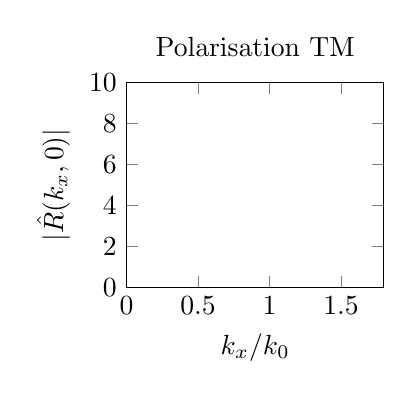
\begin{tikzpicture}[scale=1]
    \begin{axis}[
            title={Polarisation TM},
            ylabel={\(|\hat{R}(k_x,0)|\)},
            xlabel={\(k_x\slash k_0\)},
            width=0.4\textwidth,
            ymin=0,
            ymax=10,
            restrict y to domain=0:+4E+01,
            xmin=0,
            xmax=1.8,
            mark repeat=40,
            legend pos=outer north east
        ]
        % \addplot [color=black,mark=square*] table [col sep=comma, x={s1}, y={Abs(r_ex.tm)}] {csv/SOUDAIS/SOUDAIS.r_ex.MODE_2_TYPE_P.csv};
        % % \addlegendentry{Exact};

        % \addplot [color=blue,mark=x] table [col sep=comma, x={s1}, y={Abs(r_ibc0.tm)}] {csv/SOUDAIS/SOUDAIS.r_ibc.IBC_ibc0_SUC_F_MODE_2_TYPE_P.csv};
        % % \addlegendentry{CI0};

        % \addplot [color=red,mark=diamond*] table [col sep=comma, x={s1}, y={Abs(r_ibc3.tm)}] {csv/SOUDAIS/SOUDAIS.r_ibc.IBC_ibc3_SUC_F_MODE_2_TYPE_P.csv};
        % % \addlegendentry{CI3};
    \end{axis}
\end{tikzpicture}
\tikzsetnextfilename{R_SOUDAIS_plan_hoibc.TE}
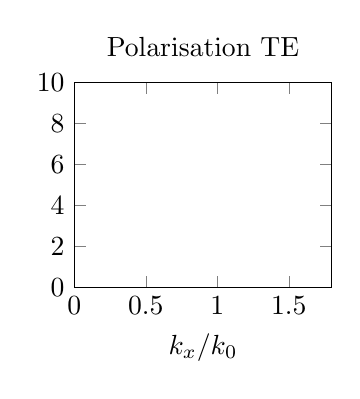
\begin{tikzpicture}[scale=1]
    \begin{axis}[
            title={Polarisation TE},
            ylabel={},
            xlabel={\(k_x\slash k_0\)},
            width=0.4\textwidth,
            xmin=0,
            xmax=1.8,
            ymin=0,
            ymax=10,
            mark repeat=40,
            legend pos=outer north east
        ]
        % \addplot [color=black,mark=square*] table [col sep=comma, x={s1}, y={Abs(r_ex.te)}] {csv/SOUDAIS/SOUDAIS.r_ex.MODE_2_TYPE_P.csv};
        % \addlegendentry{Exact};

        % \addplot [color=blue,mark=x] table [col sep=comma, x={s1}, y={Abs(r_ibc0.te)},color=] {csv/SOUDAIS/SOUDAIS.r_ibc.IBC_ibc0_SUC_F_MODE_2_TYPE_P.csv};
        % \addlegendentry{CI0};

        % \addplot [color=red,mark=diamond*] table [col sep=comma, x={s1}, y={Abs(r_ibc3.te)}] {csv/SOUDAIS/SOUDAIS.r_ibc.IBC_ibc3_SUC_F_MODE_2_TYPE_P.csv};
        % \addlegendentry{CI3};
    \end{axis}
\end{tikzpicture}
          \caption[CIOE sur empilement de P.~Soudais p.~11]{Module des coefficients diagonaux de \(\mR\) pour \(\eps = 4, \mu = 1, d=0.035\text{m}, f=12\text{GHz}\)}
          \label{fig:reflex_fourier:plan:soudais:hoibc}
      \end{figure}

      La figure \ref{fig:imp_fourier:plan:triple_asymptote:hoibc} montre la limite de la CI3 pour capturer 3 asymptotes. Pour cela, il faudrait utiliser une CI d'ordre au moins 6.

      L'expression de cette CIOE que l'on nomme \hyperlink{ci7}{CI7} est
      \begin{equation}
        \left(\oI + \sum_{i=1}^3 \left(d_{i} \left(\frac{\LD}{k_0^2}\right)^i + e_{i} \left(-\frac{\LR}{k_0^2}\right)^i \right)\right)\vE_t = \left(a_0 \oI + \sum_{i=1}^3 \left(b_{i} \left(\frac{\LD}{k_0^2}\right)^i + c_{i} \left(-\frac{\LR}{k_0^2}^i\right) \right)\right)\vJ
      \end{equation}

      \begin{figure}[!hbt]
          \centering
          \tikzsetnextfilename{Z_triple_asymptote_plan_hoibc_TM}
\begin{tikzpicture}[scale=1]
    \begin{axis}[
            title={Polarisation TM},
            ylabel={\(\Im(\hat{Z}(k_x,0)\)},
            xlabel={\(k_x\slash k_0\)},
            width=0.4\textwidth,
            xmin=0,
            xmax=1.999,
            ymin=-10,
            ymax=10,
            restrict y to domain=-300:300,
            mark repeat=200,
            legend pos=outer north east
        ]
        \addplot [color=black,mark=square*] table [col sep=comma, x={s1}, y={Im(z_ex.tm)}] {csv/triple_asymptote/triple_asymptote.z_ex.P.csv};
        % \addlegendentry{Exact};

        \addplot [color=blue,mark=x] table [col sep=comma, x={s1}, y={Im(z_ibc0.tm)}] {csv/triple_asymptote/triple_asymptote.z_ibc.IBC_ibc0_TYPE_P_SUC_F.csv};
        % \addlegendentry{CI0};

        \addplot [color=red,mark=diamond*] table [col sep=comma, x={s1}, y={Im(z_ibc3.tm)}] {csv/triple_asymptote/triple_asymptote.z_ibc.IBC_ibc3_TYPE_P_SUC_F.csv};
        % \addlegendentry{CI3};

        \addplot [color=cyan,mark=pentagon*] table [col sep=comma, x={s1}, y={Im(z_ibc7.tm)}] {csv/triple_asymptote/triple_asymptote.z_ibc.IBC_ibc7_TYPE_P_SUC_F.csv};
        % \addlegendentry{CI7};
    \end{axis}
\end{tikzpicture}
\tikzsetnextfilename{Z_triple_asymptote_plan_hoibc_TE}
\begin{tikzpicture}[scale=1]
    \begin{axis}[
            title={Polarisation TE},
            ylabel={},
            xlabel={\(k_x\slash k_0\)},
            width=0.4\textwidth,
            xmin=0,
            xmax=1.999,
            ymin=-10,
            ymax=10,
            restrict y to domain=-300:300,
            mark repeat=200,
            legend pos=outer north east
        ]
        \addplot [color=black,mark=square*] table [col sep=comma, x={s1}, y={Im(z_ex.te)}] {csv/triple_asymptote/triple_asymptote.z_ex.P.csv};
        \addlegendentry{Exact};

        \addplot [color=blue,mark=x] table [col sep=comma, x={s1}, y={Im(z_ibc0.te)}] {csv/triple_asymptote/triple_asymptote.z_ibc.IBC_ibc0_TYPE_P_SUC_F.csv};
        \addlegendentry{CI0};

        \addplot [color=red,mark=diamond*] table [col sep=comma, x={s1}, y={Im(z_ibc3.te)}] {csv/triple_asymptote/triple_asymptote.z_ibc.IBC_ibc3_TYPE_P_SUC_F.csv};
        \addlegendentry{CI3};

        \addplot [color=cyan,mark=pentagon*] table [col sep=comma, x={s1}, y={Im(z_ibc7.te)}] {csv/triple_asymptote/triple_asymptote.z_ibc.IBC_ibc7_TYPE_P_SUC_F.csv};
        \addlegendentry{CI7};                  
    \end{axis}
\end{tikzpicture}
          \caption[CIOE sur empilement avec triple asymptote]{Partie imaginaire des coefficients diagonaux de \(\mZ\) pour \(\eps = 4, \mu = 1, d=0.2\text{m}, f=1\text{GHz}\)}
          \label{fig:imp_fourier:plan:triple_asymptote:hoibc}
      \end{figure}
      \begin{table}[!hbt]
        \centering
        \begin{minipage}[t]{0.49\textwidth}
        \vspace{0pt}
        \centering
        \begin{coefftable}{\hyperlink{ci0}{CI0}}
          \input{csv/triple_asymptote/triple_asymptote.IBC_ibc0_SUC_F_MODE_2_TYPE_P.coeff.txt}
        \end{coefftable}

        \begin{coefftable}{\hyperlink{ci3}{CI3}}
          \input{csv/triple_asymptote/triple_asymptote.IBC_ibc3_SUC_F_MODE_2_TYPE_P.coeff.txt}
        \end{coefftable}
        \end{minipage}
        \tablecoeff[0.49]{\hyperlink{ci7}{CI7}}{csv/triple_asymptote/triple_asymptote.IBC_ibc7_SUC_F_MODE_2_TYPE_P.coeff.txt}
        \caption{Coefficients associés à la figure \ref{fig:imp_fourier:plan:triple_asymptote:hoibc}}
        \label{tab:imp_fourier:plan:triple_asymptote:hoibc}
      \end{table}
      Il faut donc une CIOE d'ordre 2 fois le nombre d'asymptote que l'on rencontre sur notre balayage.



\sectionstar{Conclusion}
Nous avons montré comment calculer les coefficients dans le cas d'un objet sphérique en minimisant au sens des moindres carrés la différence entre les coefficients de Mie exact et approchés. 


